\documentclass[10pt,a4paper]{article}

% ------------------------------------------------------------------
% Packages
% ------------------------------------------------------------------
\usepackage[utf8]{inputenc}
\usepackage[T1]{fontenc}
\usepackage{lmodern}
\usepackage[margin=2.2cm]{geometry}
\usepackage{amsmath,amssymb}
\usepackage{graphicx}
\usepackage{booktabs}
\usepackage{multirow}
\usepackage{tabularx}
\usepackage{array}
\usepackage{xcolor}
\usepackage[version=4]{mhchem}
\usepackage{caption}
\usepackage{subcaption}
\usepackage{tikz}
\usetikzlibrary{arrows.meta,positioning}
\usepackage[numbers,sort&compress]{natbib}
\usepackage[colorlinks=true,linkcolor=blue!50!black,citecolor=blue!50!black,urlcolor=blue!50!black]{hyperref}
\usepackage[capitalise]{cleveref}

\captionsetup{font=small,labelfont=bf}
\newcolumntype{L}{>{\raggedright\arraybackslash}X}
\newcommand{\degC}{\ensuremath{^{\circ}}C}

% ------------------------------------------------------------------
% Reported metrics. Every number in the Results section is defined
% here; update these values when the models are retrained.
% ------------------------------------------------------------------
% Nested, paper-grouped cross-validation (10_f1_improved.py, 5 outer seeds)
\newcommand{\FoneCtwo}{0.687}        \newcommand{\FoneCtwoSD}{0.042}
\newcommand{\FoneCtwoW}{0.741}       \newcommand{\BaseCtwo}{0.420}
\newcommand{\FoneCthreeP}{0.517}     \newcommand{\FoneCthreePSD}{0.040}
\newcommand{\FoneCthreePW}{0.834}    \newcommand{\BaseCthreeP}{0.310}
\newcommand{\FoneCthreeY}{0.459}     \newcommand{\FoneCthreeYSD}{0.027}
\newcommand{\FoneCthreeYW}{0.503}    \newcommand{\BaseCthreeY}{0.240}
\newcommand{\FoneCfourY}{0.398}      \newcommand{\FoneCfourYSD}{0.038}
\newcommand{\FoneCfourYW}{0.491}     \newcommand{\BaseCfourY}{0.180}
\newcommand{\FoneCfiveP}{0.355}      \newcommand{\FoneCfivePSD}{0.036}
\newcommand{\FoneCfivePW}{0.466}     \newcommand{\BaseCfiveP}{0.141}
% Surrogate regression (08_genetic algorithms.py, 80/20 split)
\newcommand{\ConvRMSE}{3.08}   \newcommand{\ConvRsq}{-0.91}
\newcommand{\YldRMSE}{11.98}   \newcommand{\YldRsq}{-0.05}

% ------------------------------------------------------------------
\title{\textbf{Machine-Learning-Guided Performance Classification and\\
Multiobjective Optimization of the Electrochemical Oxidation of\\
5-Hydroxymethylfurfural to 2,5-Furandicarboxylic Acid}}

\author{Nishit Garg\\[2pt]
\small [Affiliation]\\
\small \texttt{[email]}}

\date{}

\begin{document}
\maketitle

% ==================================================================
\begin{abstract}
\noindent
The electrochemical oxidation of 5-hydroxymethylfurfural (HMF) to
2,5-furandicarboxylic acid (FDCA) couples biomass valorization with hydrogen
evolution, but the space of catalysts, electrolytes, cell architectures and
operating conditions is too large for trial-and-error exploration. We compiled
a literature dataset of 154 electro-oxidation records from 99 publications in
43 journals and built an end-to-end machine-learning workflow comprising
leakage-controlled feature construction, K-means performance-space analysis,
SMOTE/ADASYN oversampling, classifier benchmarking, SHAP interpretation and
NSGA-II multiobjective optimization. Performance classes were defined directly
from reported HMF conversion and FDCA yield, and every classifier was evaluated
by nested cross-validation in which all records from one publication are held
out together. Combining a screen of 278 pipelines (twelve model families, five
resampling strategies) with decision rules tuned for macro-F1, regress-then-bin
classifiers and soft-vote ensembles, the selected models reach a macro-F1 of
\FoneCtwo{}\,$\pm$\,\FoneCtwoSD{} for discriminating high-performance
($\geq$90\%) systems, against \BaseCtwo{} for a majority-class predictor, and a
macro-F1 of \FoneCthreeP{} (weighted-F1 \FoneCthreePW{}) on the three-class
scheme of the reference methodology. Random-forest surrogates coupled with
NSGA-II (population 100, 100 generations) produced a fully populated
four-objective Pareto front within 0.2~min; the best-compromise candidate
combines a Ni--Cu, carbon-supported, nanostructured LDH anode descriptor set
with an alkaline \ce{OH-} electrolyte, TEMPO mediation and a flow-cell
configuration at 9.4\,\degC{} and 1.44~V, with predicted conversion of 99.3\%
and FDCA yield of 96.3\%. The workflow provides a reproducible, publication-aware
baseline for data-driven screening of HMF electro-oxidation systems.
\end{abstract}

\noindent\textbf{Keywords:} 5-hydroxymethylfurfural; 2,5-furandicarboxylic
acid; electrocatalysis; machine learning; imbalanced classification; nested
cross-validation; NSGA-II

% ==================================================================
\section{Introduction}
\label{sec:intro}

FDCA is a bio-based diacid identified among the top value-added chemicals from
biomass~\cite{werpy2004top} and a direct replacement for terephthalic acid in
polyethylene furanoate (PEF). Thermocatalytic HMF oxidation typically relies on
noble metals, pressurized \ce{O2} and elevated temperatures~\cite{sajid2018fdca}.
Electrochemical oxidation offers an attractive alternative: it proceeds at
ambient temperature and pressure, uses water as the oxygen source, and can be
paired with cathodic hydrogen evolution~\cite{cha2015combined,you2016simultaneous}.
Earth-abundant Ni, Co and Fe (oxy)hydroxides have emerged as particularly
active anodes~\cite{taitt2019comparative}. The resulting literature is large but
heterogeneous: catalysts, supports, electrolytes, cell geometries and control
modes (potentiostatic, galvanostatic or cell-voltage) vary from study to study.

Machine learning (ML) can extract structure from such literature datasets and
guide experimental design~\cite{butler2018ml}. Li~et~al.~\cite{li2025hmf}
recently demonstrated an integrated workflow for thermocatalytic HMF oxidation
in which K-means clustering defines performance classes, SMOTE~\cite{chawla2002smote}
and ADASYN~\cite{he2008adasyn} rebalance them, decision-tree, support-vector,
random-forest and neural-network classifiers are compared, SHAP~\cite{lundberg2017shap}
explains the learned models, and a genetic algorithm searches for optimal
catalyst--condition combinations.

Here we adapt this workflow to the \emph{electrochemical} route. Three aspects
of the adaptation are central. First, the electrochemical literature does not
report pressure or reaction time in a comparable form, so the descriptor set
and optimization objectives are re-formulated around electrode potential,
temperature, electrolyte and cell architecture rather than imputed. Second,
because several records usually originate from the same publication, all
evaluations hold out entire publications so that reported scores measure
generalization to unseen studies. Third, model selection is nested inside the
cross-validation so that the reported F1 scores are not inflated by choosing
the best of many pipelines on the same folds~\cite{varma2006bias,cawley2010overfitting}.

% ==================================================================
\section{Methods}
\label{sec:methods}

\subsection{Dataset compilation}
\label{sec:data}

The dataset comprises 154 records of HMF electro-oxidation extracted from 99
peer-reviewed publications in 43 journals; the most frequent sources are
\emph{Angew.\ Chem.\ Int.\ Ed.}\ (20 records), \emph{ACS Catal.}\ (14) and
\emph{Appl.\ Catal.\ B} (14). Each record contains the journal, publication
title, cell type, catalyst description (anode and counter electrode), electrolyte,
HMF concentration, applied potential or current, temperature, TEMPO mediation,
and the reported outcomes: HMF conversion, FDCA yield, faradaic efficiency (FE)
and FDCA selectivity. FDCA is the target product in 148 records; the remainder
report FFCA, DFF or 2,5-furandicarbaldehyde as the major product.

\Cref{tab:variables} summarizes the numerical variables. Outcome coverage is
incomplete: FDCA yield is reported in 123 records, conversion in 117 and both
in 102 (\cref{fig:coverage}). Operating variables are also unevenly reported;
in particular, current is available for only 15 records, reflecting the
predominance of potentiostatic studies.

\begin{table}[t]
\centering
\caption{Numerical variables of the curated dataset (154 records). $n$ is the
number of records reporting the variable.}
\label{tab:variables}
\small
\begin{tabular}{llrrrr}
\toprule
Variable & Unit & $n$ & Min & Median & Max \\
\midrule
\multicolumn{6}{l}{\emph{Operating conditions}}\\
HMF concentration         & mM            & 148 & 0.5  & 10.0  & 650 \\
Electrolyte concentration & M             & 144 & 0.1  & 1.0   & 5.0 \\
Electrode potential       & V             & 129 & 0.47 & 1.45  & 2.00 \\
Temperature               & \degC         & 91  & 2    & 25    & 60 \\
Current                   & mA            & 15  & 0.44 & 50    & 600 \\
\midrule
\multicolumn{6}{l}{\emph{Outcomes}}\\
HMF conversion            & \%            & 117 & 8.0  & 99.9  & 100 \\
FDCA yield                & \%            & 123 & 1.6  & 95.9  & 100 \\
Faradaic efficiency       & \%            & 119 & 1.6  & 95.3  & 100 \\
FDCA selectivity          & \%            & 91  & 1.6  & 98.0  & 100 \\
\bottomrule
\end{tabular}
\end{table}

\begin{figure}[t]
\centering
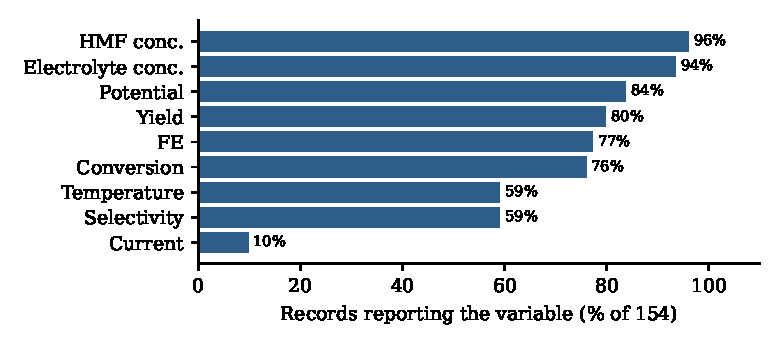
\includegraphics[width=0.72\linewidth]{figures/coverage.pdf}
\caption{Fraction of the 154 records that report each variable.}
\label{fig:coverage}
\end{figure}

\subsection{Feature construction}
\label{sec:features}

Free-text fields were converted to numerical descriptors in a single
preprocessing step, implemented in \texttt{01\_preprocess\_data.py}.

\paragraph{Electrochemical regime.} Potentials were extracted only from
potential expressions; current-density and galvanostatic expressions were routed
to a separate current variable so that applied current is never interpreted as
a potential. Binary flags record whether the potential is referenced to RHE
(122 records), whether the experiment is current-controlled (16) and whether a
cell voltage rather than an electrode potential is reported (13).

\paragraph{Catalyst.} Element flags (Ni 63, Co 28, Cu 16, Fe 11, Mo 5 records,
and $\leq$3 records each for Pd, Au, Ru, Ir, Mn, W, Ce and Ag) and material-family
flags (oxide 31, carbon 35, hydroxide 17, nanoparticle 15, oxyhydroxide 12,
LDH 10) were parsed from the catalyst description. Of the 74 records with a Pt
flag, 71 refer to a Pt counter electrode and only 3 to a Pt-containing anode;
the flag is therefore interpreted as a descriptor of the electrode assembly
rather than of the anode catalyst.

\paragraph{Electrolyte and cell.} Electrolyte concentration, an alkalinity flag
(136 records), anion flags (\ce{OH-} 136, \ce{ClO4-} 4, \ce{SO4^2-} 3,
\ce{HCO3-} 2, unspecified 9), TEMPO mediation (8) and cell-architecture flags
(divided 90, three-electrode 22, flow 12, undivided 8) complete the descriptor
set.

\paragraph{Engineered descriptors.} For classification, these were augmented
with the logarithm of HMF concentration, the HMF-to-electrolyte ratio,
potential--regime interactions, noble/base-metal indicators and the number of
distinct metals, giving 72 input features (\texttt{09\_f1\_optimization.py}).
In the final models (\texttt{10\_f1\_improved.py}), the Pt flag is replaced by an
anode-only Pt flag, the noble-metal indicator and metal count are recomputed
accordingly, and three flags record whether temperature, potential and current
are reported, giving 73 features.

\paragraph{Leakage control.} Conversion, yield, FE and selectivity are never
used as inputs, nor are free-text fields that describe outcomes (key feature,
advantages, limitations). The publication title is used only as a grouping
variable for cross-validation.

\subsection{Performance-space analysis}
\label{sec:kmeans}

Following the reference methodology~\cite{li2025hmf}, K-means
clustering~\cite{lloyd1982kmeans} was applied to standardized conversion and
yield for the 102 complete records with $K = 3$--$6$ to map the structure of
the performance space (\texttt{02\_kmeans.py}). The clusters describe
performance regions rather than catalyst families. Their visualization after
SMOTE and ADASYN rebalancing is provided by \texttt{04\_kmeans\_oversampling.py}.

\subsection{Performance classes}
\label{sec:classes}

For each record that reports a yield, a single performance score is defined as
\begin{equation}
  P = \begin{cases}
      \min(X_{\text{HMF}},\, Y_{\text{FDCA}}) & \text{if conversion } X_{\text{HMF}} \text{ is reported},\\
      Y_{\text{FDCA}} & \text{otherwise},
      \end{cases}
  \label{eq:perf}
\end{equation}
which uses the fact that yield cannot exceed conversion. This raises the number
of usable records from 102 to 123. Five class schemes were evaluated
(\cref{tab:classes,fig:classes}), so that conclusions do not depend on a single
choice of thresholds. C3-P uses the thresholds of the reference
methodology~\cite{li2025hmf}.

\begin{table}[t]
\centering
\caption{Performance-class schemes ($n = 123$). $P$ is defined in \cref{eq:perf}
and $Y$ is FDCA yield.}
\label{tab:classes}
\small
\begin{tabular}{lllr}
\toprule
Scheme & Basis & Class boundaries (\%) & Class sizes \\
\midrule
C2   & $P$ & $<$90, $\geq$90                 & 34 / 89 \\
C3-P & $P$ & $<$50, 50--80, $\geq$80         & 9 / 7 / 107 \\
C3-Y & $Y$ & $<$80, 80--95, $\geq$95         & 16 / 38 / 69 \\
C4-Y & $Y$ & $<$50, 50--80, 80--95, $\geq$95 & 9 / 7 / 38 / 69 \\
C5-P & $P$ & $<$50, 50--80, 80--90, 90--95, $\geq$95 & 9 / 7 / 18 / 22 / 67 \\
\bottomrule
\end{tabular}
\end{table}

\begin{figure}[t]
\centering
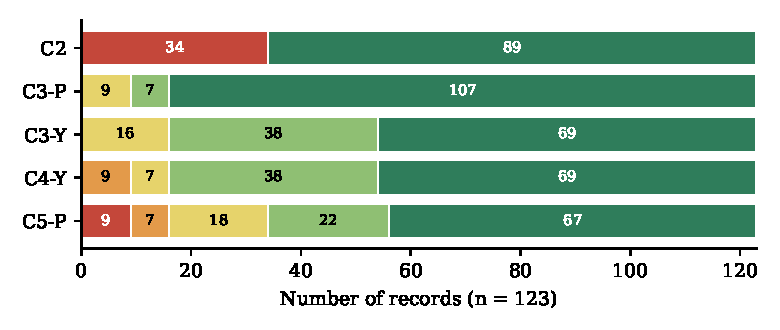
\includegraphics[width=0.72\linewidth]{figures/class_distribution.pdf}
\caption{Class sizes for the five schemes, ordered from the lowest (left) to the
highest (right) performance class.}
\label{fig:classes}
\end{figure}

\subsection{Classification pipelines}
\label{sec:pipelines}

Each pipeline consists of median imputation, standardization, optional
univariate feature selection (top 20 features by ANOVA $F$-score, or all 72),
optional resampling and a classifier, implemented in
scikit-learn~\cite{pedregosa2011sklearn} and imbalanced-learn~\cite{lemaitre2017imblearn}.
Resampling options are none, SMOTE~\cite{chawla2002smote}, Borderline-SMOTE~\cite{han2005borderline},
ADASYN~\cite{he2008adasyn} and random oversampling; the neighbourhood size of
the synthetic samplers is reduced automatically when a minority class is smaller
than the default. Twelve classifier families were considered: decision tree,
random forest~\cite{breiman2001rf} and extra trees~\cite{geurts2006extra} (each
with and without class weighting where applicable), gradient boosting,
support-vector machine, logistic regression, $k$-nearest neighbours and
multilayer-perceptron neural networks, each with several hyper-parameter
settings. In total, 278 pipelines were evaluated per class scheme.

Resampling and feature selection are fitted inside each training fold only, so
synthetic records never enter a test fold.

\subsection{Decision rules and final model pool}
\label{sec:rules}

Predicting the most probable class favours the dominant class and does not
maximize macro-F1. The final model pool therefore pairs each model with a
decision rule tuned for macro-F1:
\begin{itemize}
\item \emph{Classifiers} (class-weighted random forest, extra trees,
  support-vector machine and logistic regression; gradient boosting,
  $k$-nearest neighbours and a neural network with or without SMOTE) output
  class probabilities $p_c$, and the predicted class is
  $\arg\max_c w_c\, p_c$, with per-class weights $w_c$ found by coordinate
  ascent.
\item \emph{Regress-then-bin} models (random forest, extra trees, gradient
  boosting with Huber loss, ridge regression and support-vector regression)
  predict the continuous quantity from which the classes are defined ($P$, or
  $Y$ for the yield-based schemes), which is then cut into classes at ordered
  cut-offs found by coordinate ascent. These models learn from the full
  outcome scale rather than from class labels alone.
\item A \emph{soft-vote ensemble} averages the probabilities of the three best
  classifiers and tunes its own class weights.
\end{itemize}
The pool contains 44 candidates: 19 models, each with all 73 features or the
top 20, with gradient boosting, $k$-nearest neighbours and the neural network
also run with and without SMOTE.
Weights and cut-offs are tuned on inner out-of-fold predictions (two repeats of
three-fold grouped cross-validation) and are then frozen before the outer test
fold is predicted.

\subsection{Validation protocol}
\label{sec:validation}

All splits are stratified by class and grouped by publication
(\texttt{StratifiedGroupKFold}), so that records from a given study never
appear in both training and test data.

\paragraph{Screening.} Each pipeline is scored by five repetitions of
five-fold grouped cross-validation.

\paragraph{Nested evaluation.} Within each outer training fold, every candidate
in the pool, together with its tuned decision rule, is ranked by inner grouped
cross-validation; the best candidate (or the ensemble, if it ranks higher) is
refitted on the outer training fold and scored on the held-out publications.
The outer loop uses five folds and is repeated with five random seeds. Scores
from this procedure are the headline results, because selecting the best of
many pipelines on the same folds is optimistically
biased~\cite{varma2006bias,cawley2010overfitting}. The same nested procedure
applied to the 278-pipeline screen with plain most-probable-class prediction
serves as the reference protocol.

\paragraph{Metrics.} The primary metric is macro-averaged F1, which weights all
classes equally and is therefore sensitive to the minority classes; the
support-weighted F1 is also reported~\cite{sokolova2009systematic}. A
majority-class predictor provides the reference level for each scheme.

\subsection{Surrogate models and NSGA-II optimization}
\label{sec:nsga}

For optimization, separate random-forest regressors (300 trees, minimum leaf
size 2) predict HMF conversion and FDCA yield from 30 descriptors: five
continuous variables (HMF concentration, electrolyte concentration, potential,
temperature and current) and 25 binary flags. Binary flags with prevalence below
2\% or above 98\% were removed because they are unstable as free decision
variables. Missing values were median-imputed. The surrogates were validated on
an 80/20 split (81/21 records) and then refitted on all 102 complete records.

NSGA-II~\cite{deb2002nsga2} was run on four objectives: maximize predicted
conversion, maximize predicted yield, minimize temperature and minimize electrode
potential. Temperature and potential are bounded to the observed ranges of the
training records (4--60\,\degC{} and 0.47--1.90~V), and binary variables are
repaired to $\{0,1\}$ after each variation step. The population size is 100,
the number of generations 100, and the crossover and mutation rates 0.90 and
0.10. Population members are evaluated in batches. Pareto-front uniformity is
tracked with the spacing metric, and the standardized Euclidean distance from
each candidate to its nearest training record is reported as an
extrapolation diagnostic.

A single best-compromise candidate is selected from the final Pareto front by a
weighted sum of min--max-normalized objectives (0.40 conversion, 0.40 yield,
0.10 temperature, 0.10 potential). This ranking is applied after optimization
and is not an NSGA-II objective.

\begin{figure}[t]
\centering
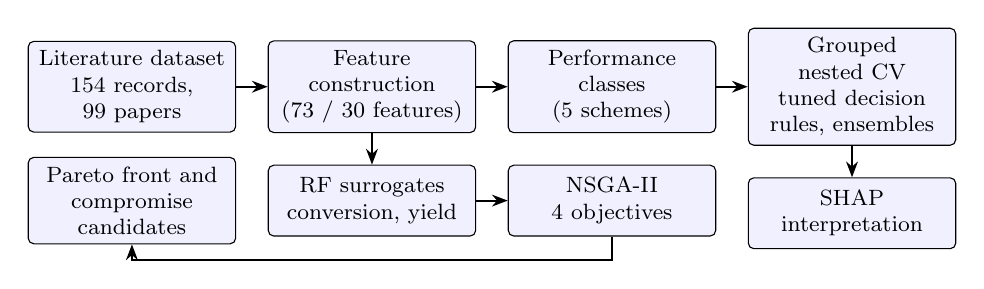
\begin{tikzpicture}[
  node distance=4mm and 4mm,
  box/.style={draw, rounded corners=2pt, fill=blue!6, align=center,
              font=\footnotesize, minimum height=9mm, text width=24mm},
  arr/.style={-{Stealth[length=2mm]}, thick}]
\node[box] (a) {Literature dataset\\154 records, 99 papers};
\node[box, right=of a] (b) {Feature\\construction\\(73 / 30 features)};
\node[box, right=of b] (c) {Performance\\classes\\(5 schemes)};
\node[box, right=of c] (d) {Grouped nested CV\\tuned decision\\rules, ensembles};
\node[box, below=of d] (e) {SHAP\\interpretation};
\node[box, below=of b] (f) {RF surrogates\\conversion, yield};
\node[box, left=of f] (g) {Pareto front and\\compromise\\candidates};
\node[box, right=of f] (h) {NSGA-II\\4 objectives};
\draw[arr] (a) -- (b); \draw[arr] (b) -- (c); \draw[arr] (c) -- (d);
\draw[arr] (d) -- (e);
\draw[arr] (b) -- (f); \draw[arr] (f) -- (h); \draw[arr] (h.south) -- ++(0,-3mm) -| (g.south);
\end{tikzpicture}
\caption{Overview of the workflow. The upper branch classifies reported
performance; the lower branch optimizes operating conditions through
random-forest surrogates and NSGA-II.}
\label{fig:workflow}
\end{figure}

% ==================================================================
\section{Results and discussion}
\label{sec:results}

\subsection{Classification performance}
\label{sec:clf}

\Cref{tab:nested} and \cref{fig:f1} report the nested, publication-grouped
scores. All five schemes exceed the majority-class baseline in macro-F1, by
0.21 (C3-P) to 0.27 (C2). The binary C2 task, which separates systems reaching
at least 90\% performance from the rest, achieves a macro-F1 of
\FoneCtwo{}\,$\pm$\,\FoneCtwoSD{}, with class-wise F1 of 0.45--0.62 for the
$<$90\% class and 0.76--0.84 for the $\geq$90\% class across seeds. On the
three-class C3-P scheme of the reference methodology, the weighted-F1 is
\FoneCthreePW{} and the F1 of the dominant $\geq$80\% class is 0.89--0.94,
while the macro-F1 of \FoneCthreeP{} reflects the difficulty of the two
minority classes with only 9 and 7 records (F1 of 0.10--0.15 and 0.36--0.63).
Macro-F1 decreases steadily as classes become finer, from \FoneCtwo{} for two
classes to \FoneCfiveP{} for five.

\paragraph{Effect of the decision rules.} \Cref{tab:improvement} compares the
final pool with the reference protocol on identical outer splits. The tuned
pool improves macro-F1 on every scheme, by 0.083 on C2, 0.042 on C3-P, 0.037
on C3-Y, 0.021 on C4-Y and 0.008 on C5-P, and improves weighted-F1 on every
scheme. The gain is largest where the decision threshold matters most: on the
binary task, reweighting moves predictions towards the minority class that
plain most-probable-class prediction under-predicts. Across the 125 outer
folds, the soft-vote ensemble was selected 40 times, followed by the neural
network (21), class-weighted extra trees (19) and class-weighted logistic
regression (12). Regress-then-bin models were selected 16 times, most often
ridge regression on C3-Y, where the classes are cut from yield alone. The seed-to-seed standard deviation of 0.03--0.04 shows
that the choice of outer split contributes uncertainty of the same order as
the smaller gains, so the C4-Y and C5-P improvements should be regarded as
indicative.

\begin{table}[t]
\centering
\caption{Nested macro-F1 (weighted-F1 in parentheses) of the reference protocol
and the final pool on identical outer splits (seeds 100 and 101).}
\label{tab:improvement}
\small
\begin{tabular}{lccc}
\toprule
Scheme & Reference protocol & Final pool & $\Delta$ macro-F1 \\
\midrule
C2   & 0.610 (0.685) & 0.693 (0.747) & +0.083 \\
C3-P & 0.460 (0.824) & 0.502 (0.829) & +0.042 \\
C3-Y & 0.445 (0.516) & 0.482 (0.531) & +0.037 \\
C4-Y & 0.367 (0.459) & 0.388 (0.487) & +0.021 \\
C5-P & 0.327 (0.426) & 0.335 (0.455) & +0.008 \\
\bottomrule
\end{tabular}
\end{table}

\begin{table}[t]
\centering
\caption{Nested cross-validation results of the final model pool with
publication-grouped splits (outer 5-fold, five seeds; inner grouped selection
and decision-rule tuning). Values are mean\,$\pm$\,s.d.\ over seeds.}
\label{tab:nested}
\small
\begin{tabular}{lcccc}
\toprule
Scheme & Classes & Macro-F1 & Weighted-F1 & Majority-class macro-F1 \\
\midrule
C2   & 2 & $\FoneCtwo \pm \FoneCtwoSD$       & \FoneCtwoW    & \BaseCtwo \\
C3-P & 3 & $\FoneCthreeP \pm \FoneCthreePSD$ & \FoneCthreePW & \BaseCthreeP \\
C3-Y & 3 & $\FoneCthreeY \pm \FoneCthreeYSD$ & \FoneCthreeYW & \BaseCthreeY \\
C4-Y & 4 & $\FoneCfourY \pm \FoneCfourYSD$   & \FoneCfourYW  & \BaseCfourY \\
C5-P & 5 & $\FoneCfiveP \pm \FoneCfivePSD$   & \FoneCfivePW  & \BaseCfiveP \\
\bottomrule
\end{tabular}
\end{table}

\begin{figure}[t]
\centering
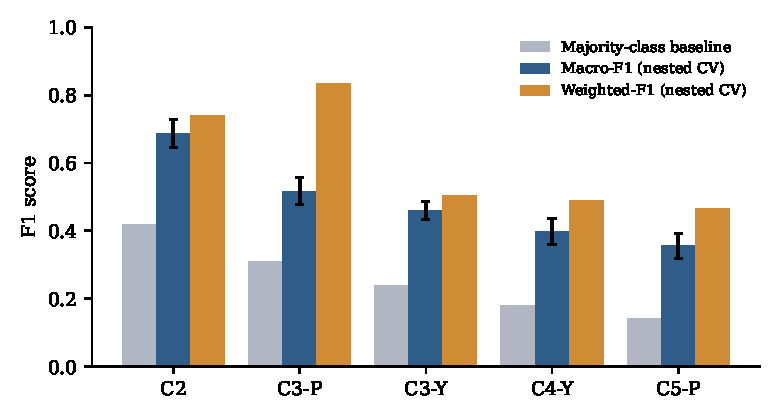
\includegraphics[width=0.72\linewidth]{figures/f1_nested.pdf}
\caption{Nested-CV macro-F1 (error bars: s.d.\ over seeds) and weighted-F1
compared with a majority-class predictor for each class scheme.}
\label{fig:f1}
\end{figure}

\paragraph{Effect of model selection.} The highest single-pipeline screening
score on C2 is 0.763 (logistic regression with ADASYN and 20 selected features),
and on C3-P it is 0.581 (extra trees with random oversampling). Under the
reference protocol the corresponding nested scores are 0.153 and 0.121 lower.
This gap is the optimism introduced by choosing one pipeline from 278 on the
same folds, and it is why nested scores are used throughout. The smaller,
rule-tuned pool of the final models halves this gap on C2 (0.076).

\paragraph{Classifier families.} \Cref{tab:families} lists the screening
macro-F1 of the four model families used in the reference
study~\cite{li2025hmf}, each with fixed default settings and SMOTE or ADASYN.
No family is uniformly best: random forest leads on C2, C3-Y and C5-P, the
neural network on C3-P and C4-Y, while the support-vector machine is weakest on
every scheme with more than two classes. The pipelines most often chosen in
the nested loop were similarly diverse (support-vector, logistic-regression,
$k$-nearest-neighbour, tree-ensemble and neural-network models), which
indicates that the achievable score is limited by the data rather than by the
model class.

\begin{table}[t]
\centering
\caption{Screening macro-F1 of the reference study's four model families with
fixed settings and SMOTE/ADASYN (5$\times$5-fold grouped CV). Bold marks the
best family per scheme.}
\label{tab:families}
\small
\begin{tabular}{lcccc}
\toprule
Scheme & Decision tree & SVM & Random forest & Neural network \\
\midrule
C2   & 0.611 & 0.543 & \textbf{0.627} & 0.597 \\
C3-P & 0.516 & 0.305 & 0.473 & \textbf{0.526} \\
C3-Y & 0.422 & 0.371 & \textbf{0.477} & 0.442 \\
C4-Y & 0.420 & 0.239 & 0.436 & \textbf{0.486} \\
C5-P & 0.282 & 0.236 & \textbf{0.398} & 0.372 \\
\bottomrule
\end{tabular}
\end{table}

\paragraph{Effect of oversampling.} \Cref{tab:sampling} compares the best
screening score obtained with each resampling strategy. Differences between
strategies are at most 0.022 macro-F1, and the best oversampler exceeds
training without resampling by at most 0.014 (C4-Y); on C2 the two are equal.
Unlike in the reference study, where oversampling substantially improved
generalization~\cite{li2025hmf}, oversampling here acts mainly as a
stabilizer: the minority classes of C3-P to C5-P contain only 7--9 records,
from only a handful of publications, so interpolated samples add little new
information about unseen studies.

\begin{table}[t]
\centering
\caption{Best screening macro-F1 by resampling strategy (maximum over
classifiers and feature-selection settings).}
\label{tab:sampling}
\small
\begin{tabular}{lccccc}
\toprule
Scheme & None & SMOTE & Borderline-SMOTE & ADASYN & Random \\
\midrule
C2   & 0.763 & 0.746 & 0.741 & 0.763 & 0.742 \\
C3-P & 0.579 & 0.581 & 0.575 & 0.578 & 0.581 \\
C3-Y & 0.516 & 0.508 & 0.514 & 0.518 & 0.525 \\
C4-Y & 0.484 & 0.491 & 0.477 & 0.498 & 0.489 \\
C5-P & 0.399 & 0.397 & 0.405 & 0.400 & 0.388 \\
\bottomrule
\end{tabular}
\end{table}

\paragraph{Comparison with the reference study.} The reference workflow reports
F1 scores of about 0.8 on 379 thermocatalytic records whose descriptors include
pressure, reaction time and alkali loading, and whose classes come from K-means
clusters~\cite{li2025hmf}. The present dataset is a third of that size,
covers a different reaction route, lacks those process variables, and is
strongly skewed: 87\% of records exceed 80\% performance. In addition, our
splits hold out whole publications, which is a stricter test than record-level
splitting. The two sets of scores therefore measure different tasks and should
not be compared directly.

\subsection{Model interpretation}
\label{sec:shap}

SHAP values~\cite{lundberg2017shap} were computed for SMOTE-balanced
neural-network classifiers at $K = 3$ and $K = 5$ (\texttt{06\_shap\_analysis.py},
\texttt{07\_shap\_extra\_figures.py}). SHAP attributions quantify the
contribution of each descriptor to the model output; they explain the fitted
model and are not, by themselves, evidence of a causal chemical effect.

\subsection{Surrogate models}
\label{sec:surrogate}

On the 21-record validation split, the random-forest surrogates reach an RMSE
of \ConvRMSE{} percentage points for conversion and \YldRMSE{} percentage points
for yield (\cref{tab:surrogate}). The negative $R^2$ values show that the
surrogates do not outperform the mean of the validation records on this split.
For conversion, this follows from the very narrow target distribution (median
99.9\%), in which a small absolute error is large relative to the variance.
For yield, the error is substantial. The surrogates therefore define a smooth
landscape for exploration, and Pareto candidates are interpreted as
hypotheses for experimental testing rather than as validated optima.

\begin{table}[t]
\centering
\caption{Random-forest surrogate validation (80/20 split, random state 42).}
\label{tab:surrogate}
\small
\begin{tabular}{lcccc}
\toprule
Target & RMSE (pp) & $R^2$ & Train $n$ & Test $n$ \\
\midrule
HMF conversion & \ConvRMSE & \ConvRsq & 81 & 21 \\
FDCA yield     & \YldRMSE  & \YldRsq  & 81 & 21 \\
\bottomrule
\end{tabular}
\end{table}

\subsection{Multiobjective optimization}
\label{sec:ga}

NSGA-II completed 100 generations in 0.17~min. The front first reached the
full population size of 100 at generation~7 and contained 89--100 members in
every later generation. The best predicted conversion rose from 98.0\% in the
first generation to 99.4\% and the best predicted yield from 89.8\% to 97.2\%;
most of the gain occurred within the first 40 generations, followed by small
increments up to generation~88 (\cref{fig:ga}b). The spacing metric fell from
0.150 in the first generation to 0.039--0.076 from generation~6 onward,
indicating an evenly spread front (\cref{fig:ga}c). Because the problem has four objectives,
the projection of the front onto the conversion--yield plane
(\cref{fig:ga}a) contains points that are non-dominated only through
temperature or potential.

\begin{figure}[t]
\centering
\begin{subfigure}{0.32\linewidth}
  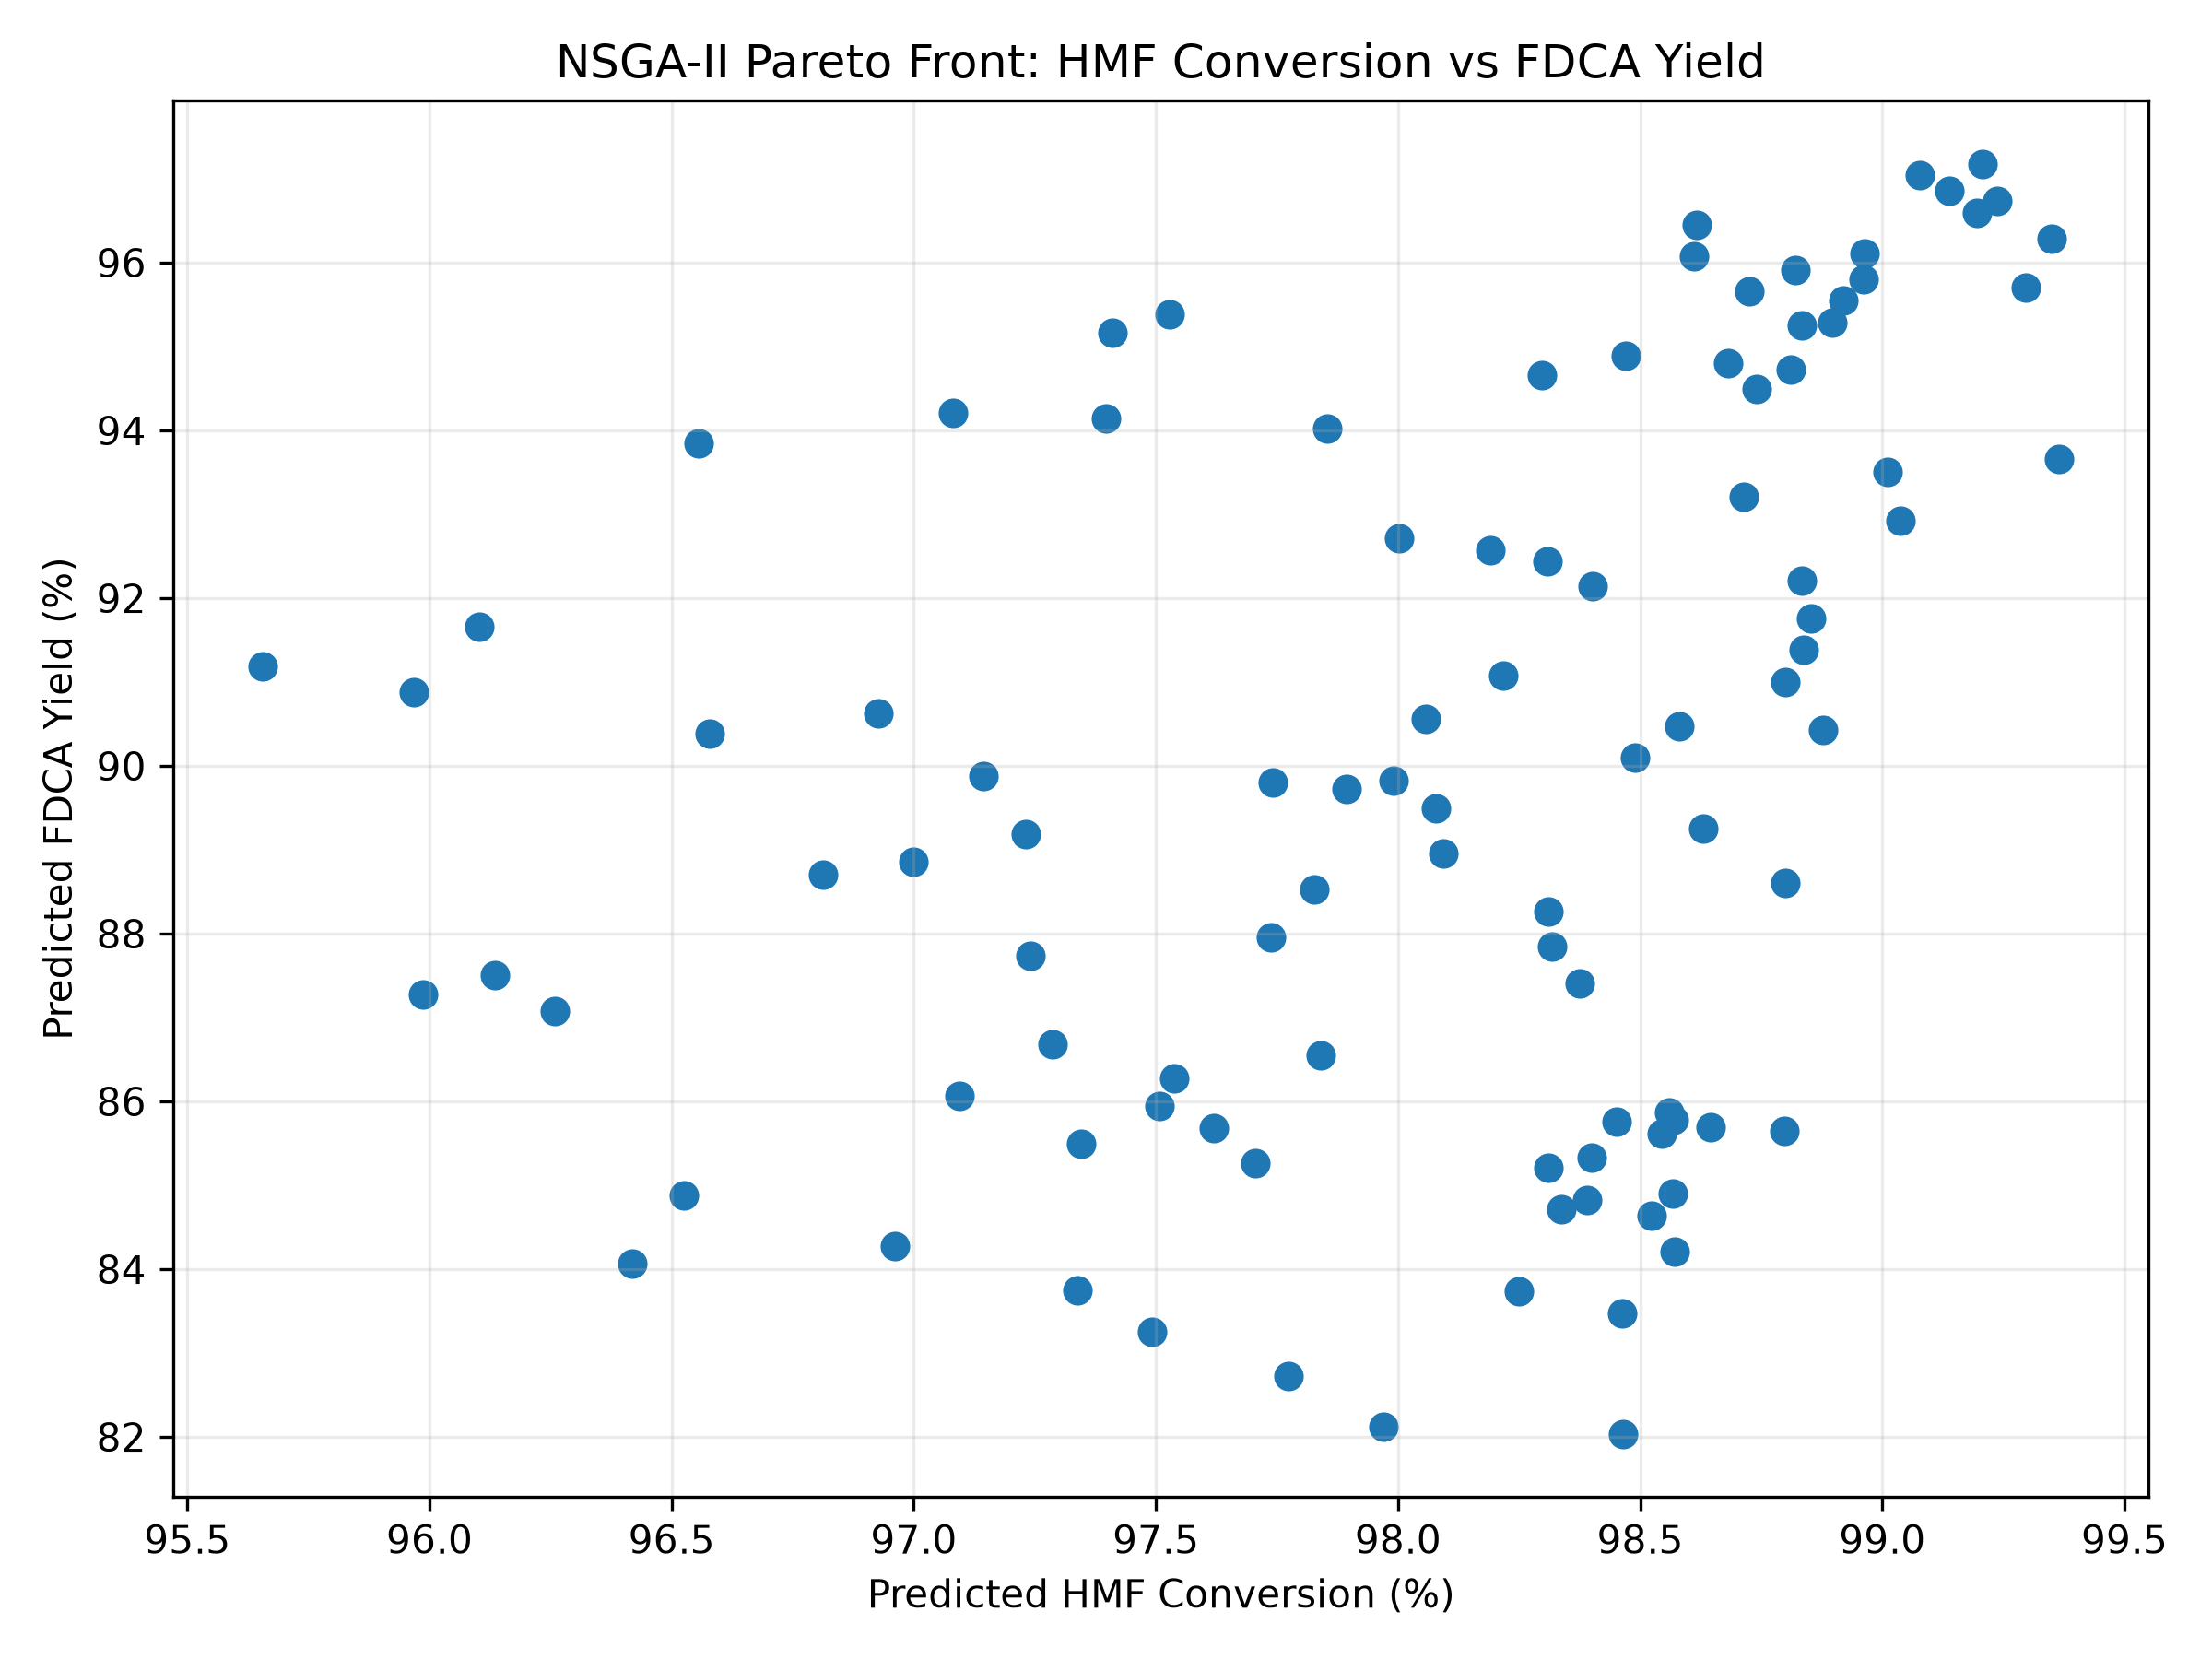
\includegraphics[width=\linewidth]{figures/NSGAII_Pareto_Front.png}
  \caption{}
\end{subfigure}\hfill
\begin{subfigure}{0.32\linewidth}
  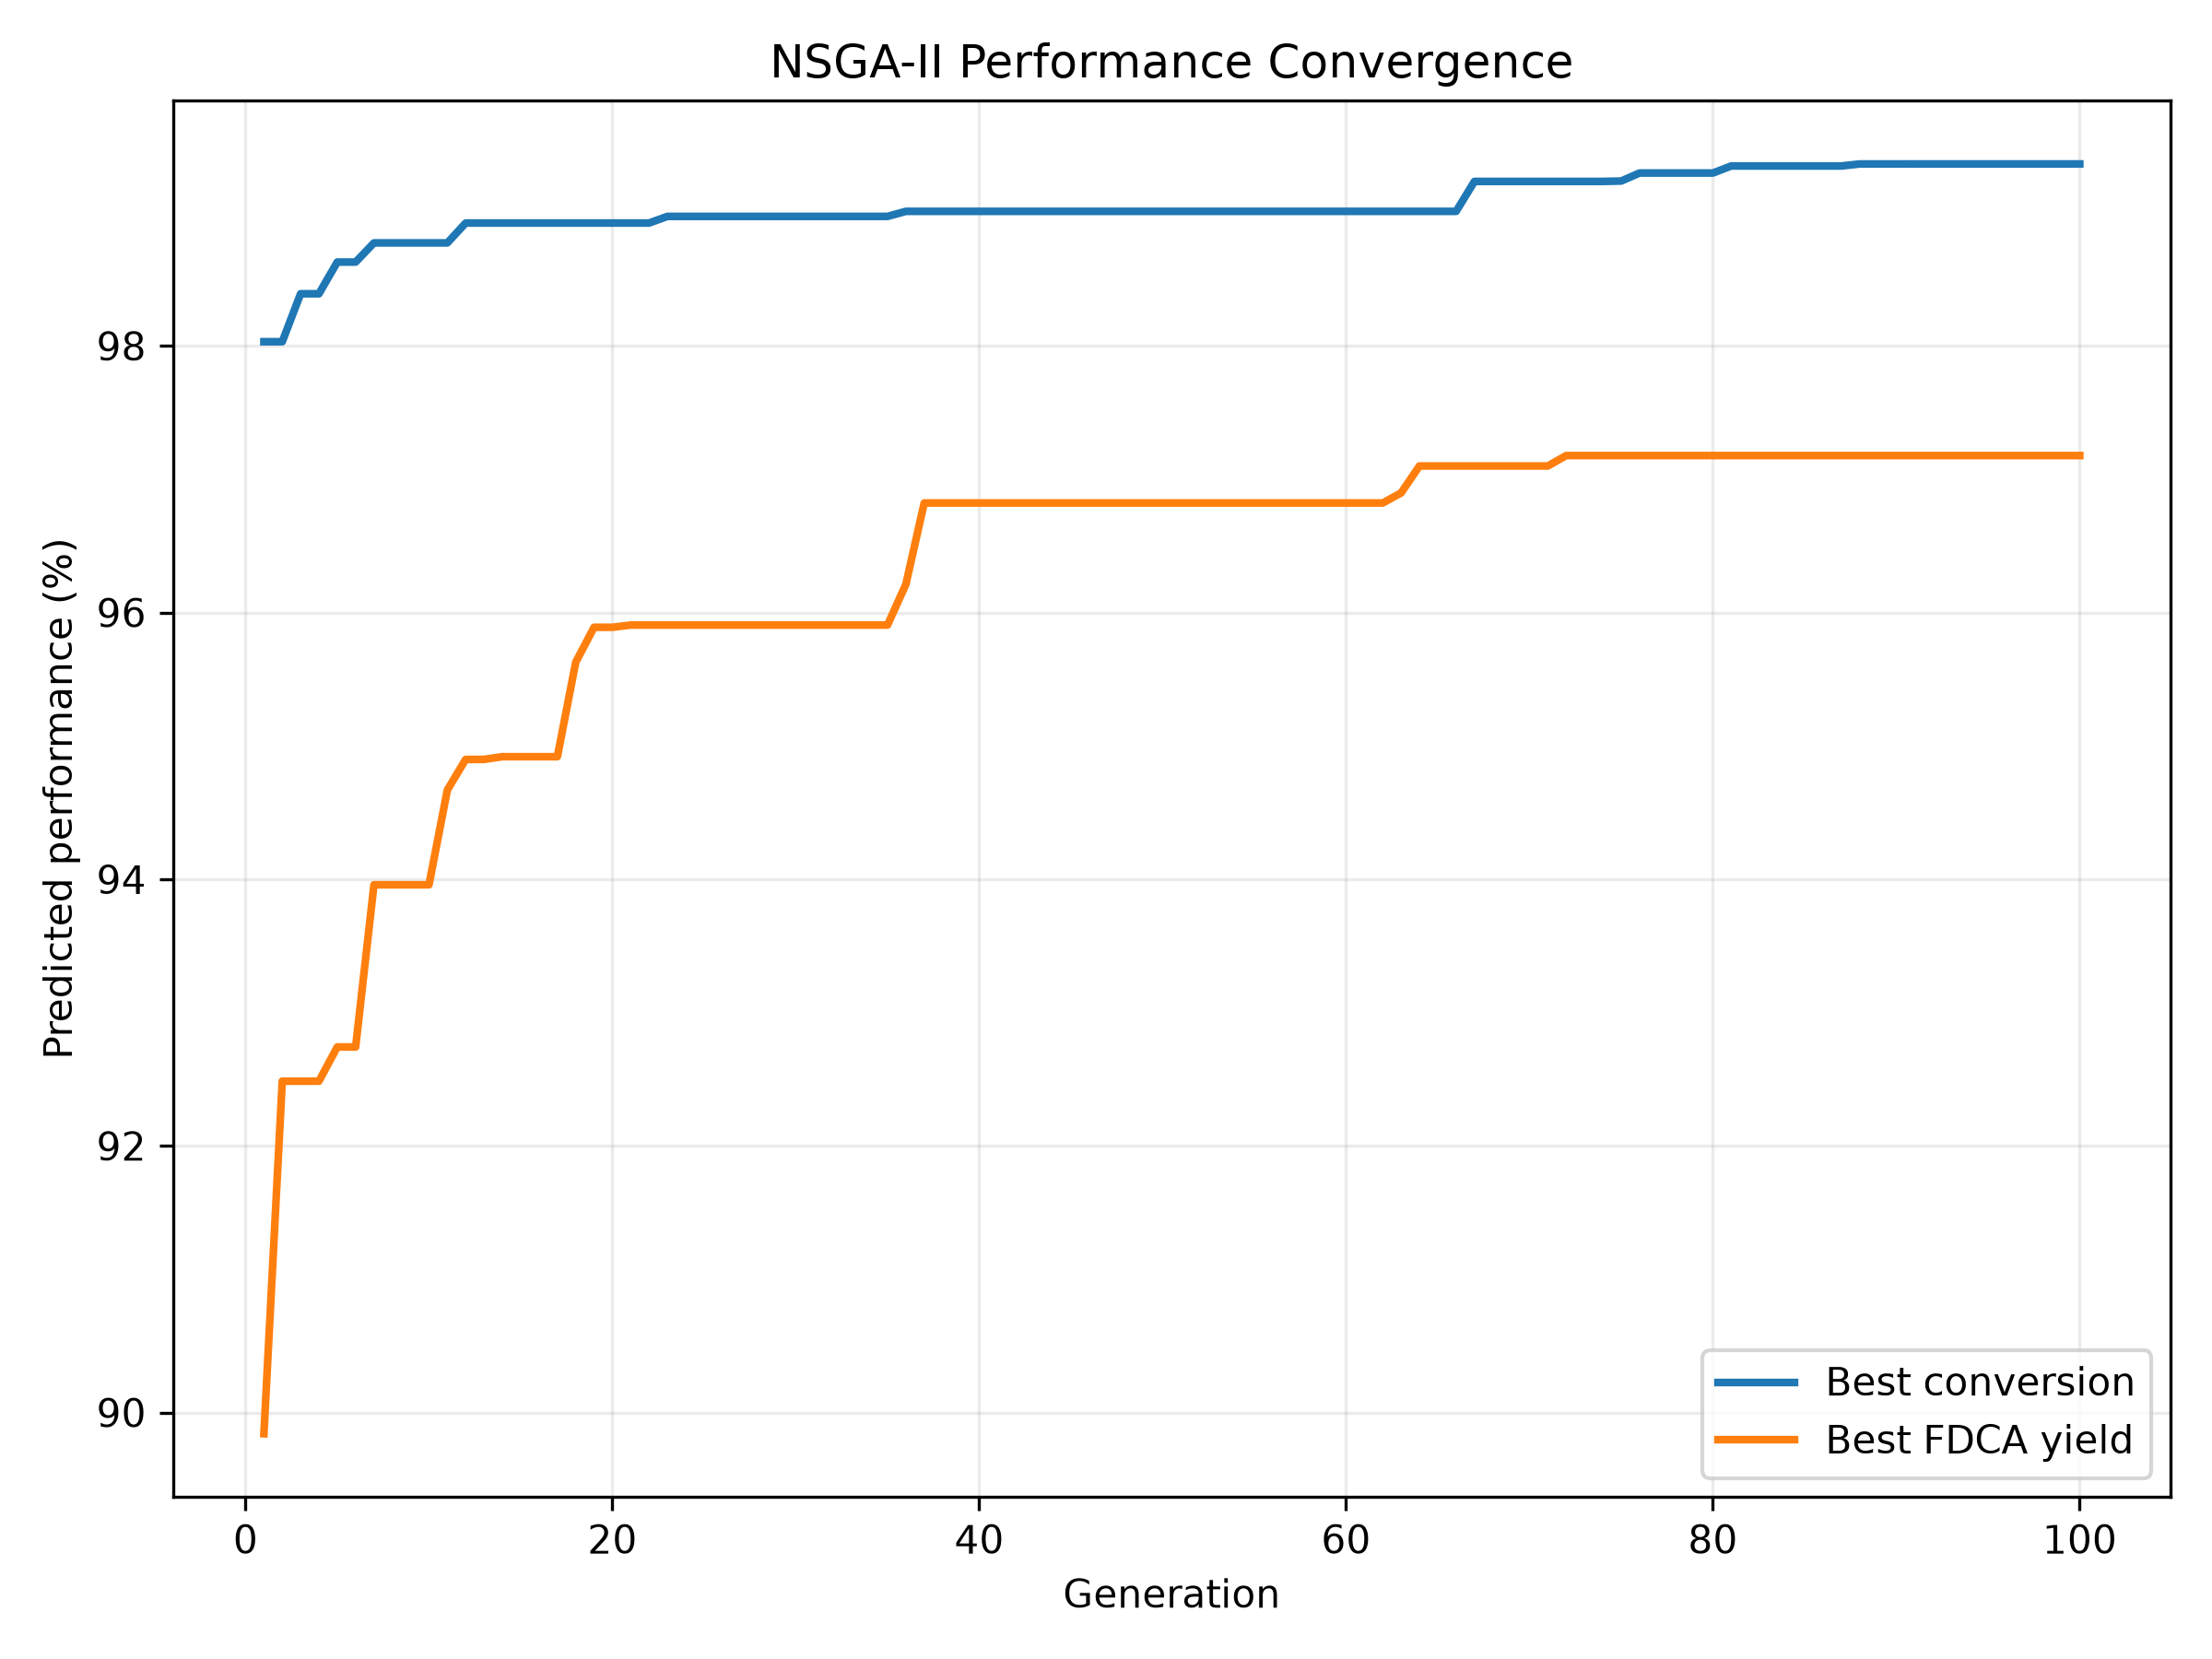
\includegraphics[width=\linewidth]{figures/NSGAII_Convergence.png}
  \caption{}
\end{subfigure}\hfill
\begin{subfigure}{0.32\linewidth}
  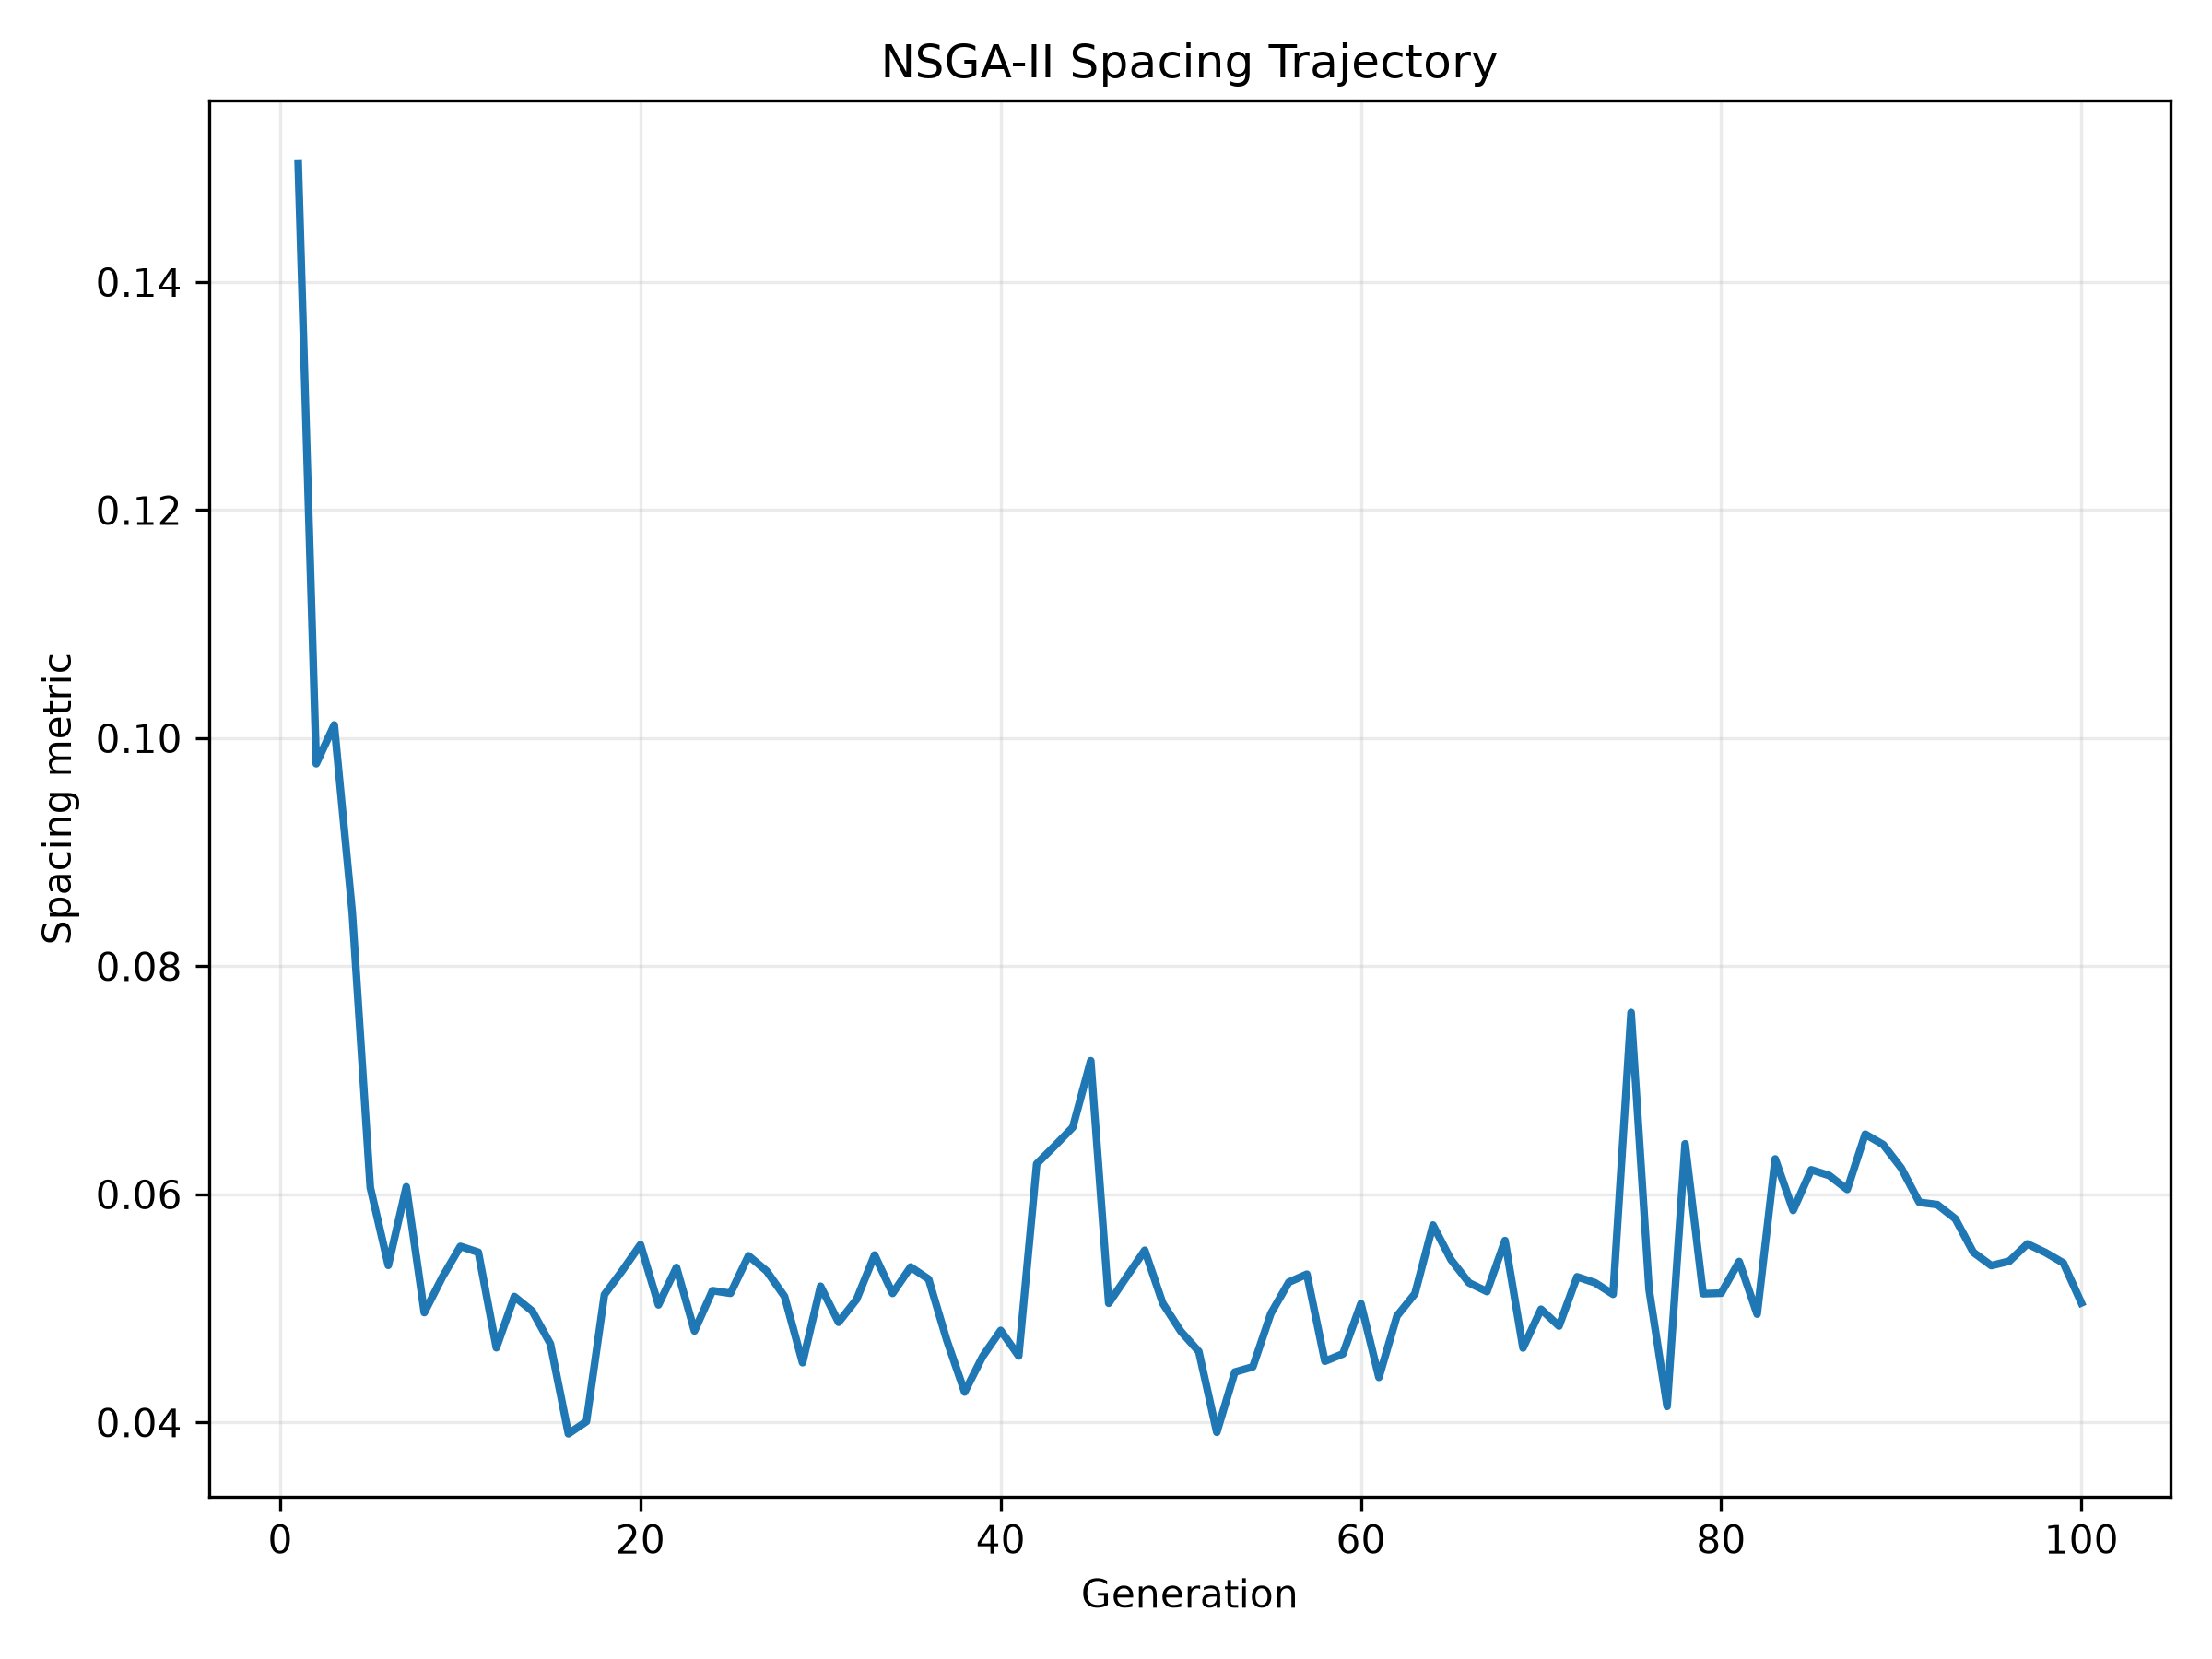
\includegraphics[width=\linewidth]{figures/NSGAII_Spacing_Trajectory.png}
  \caption{}
\end{subfigure}
\caption{NSGA-II results. (a) Final Pareto front projected onto predicted
conversion and FDCA yield. (b) Best predicted conversion and yield per
generation. (c) Spacing metric per generation.}
\label{fig:ga}
\end{figure}

\Cref{tab:pareto} lists the five highest-ranked Pareto candidates. All five
share an alkaline electrolyte, an RHE-referenced potential between 1.42 and
1.44~V, a Ni and/or Cu anode descriptor with nanoparticle morphology, and TEMPO
mediation. Predicted conversions lie between 99.1 and 99.4\% and predicted
yields between 95.7 and 96.9\%, at temperatures of 7.5--21.6\,\degC. The
best-compromise candidate (score 0.863) combines Ni, Cu, LDH, carbon and
nanoparticle descriptors in a flow cell with an \ce{OH-} electrolyte of
2.19~M, an HMF concentration of 238~mM and a current of 298~mA, operated at
9.4\,\degC{} and 1.44~V vs.\ RHE.

\begin{table*}[t]
\centering
\caption{Top five Pareto candidates ranked by the post-hoc compromise score.
Conv.\ and Yield are surrogate predictions. $d_{\min}$ is the standardized
distance to the nearest training record. All candidates use an alkaline
electrolyte, RHE-referenced potential control and TEMPO.}
\label{tab:pareto}
\footnotesize
\setlength{\tabcolsep}{4pt}
\resizebox{\textwidth}{!}{\begin{tabular}{cccccccccllllc}
\toprule
Rank & Score & Conv.\ (\%) & Yield (\%) & $T$ (\degC) & $E$ (V) & HMF (mM)
& Electrolyte (M) & $I$ (mA) & Metals & Material family & Cell & Anion & $d_{\min}$ \\
\midrule
1 & 0.863 & 99.35 & 96.29 &  9.39 & 1.441 & 237.9 & 2.19 & 297.8 & Ni, Cu & LDH, C, NP     & Flow & \ce{OH-}        & 9.44 \\
2 & 0.846 & 99.30 & 95.71 &  7.51 & 1.441 & 237.9 & 2.19 & 297.8 & Cu     & Oxide, LDH, C, NP & Flow & \ce{OH-}     & 10.00 \\
3 & 0.844 & 99.14 & 96.86 & 14.94 & 1.418 & 361.0 & 2.19 & 332.6 & Ni     & C, NP          & ---  & \ce{OH-}$^{a}$  & 9.08 \\
4 & 0.843 & 99.19 & 96.60 & 14.04 & 1.445 & 223.7 & 2.14 & 306.1 & Ni, Cu & NP             & ---  & \ce{OH-}$^{a}$  & 8.18 \\
5 & 0.836 & 99.24 & 96.73 & 21.56 & 1.418 & 185.4 & 2.30 & 304.1 & Ni, Cu & LDH, C, NP     & ---  & \ce{OH-}        & 8.38 \\
\bottomrule
\end{tabular}}

\vspace{2pt}
\raggedright\footnotesize
C = carbon, NP = nanoparticle. ``---'': no cell-architecture flag active.
$^{a}$The unspecified-anion flag is also active.
\end{table*}

Three features of the front bear on experimental follow-up. First, the leading
candidates lie at standardized distances of 8.2--10.0 from the nearest training
record. Their HMF concentrations (185--361~mM) and currents (298--333~mA) are
well above the dataset medians (10~mM and 50~mA), and current is reported in
only 15 records, so these values partly reflect median-imputed regions of the
descriptor space. Second, because binary descriptors are varied independently,
some candidates carry no cell-architecture flag (ranks 3--5) or combine the
\ce{OH-} and unspecified-anion flags (ranks 3 and 4); these are descriptor-level
patterns rather than complete experimental recipes. Third, the low predicted
optimal temperatures (7.5--21.6\,\degC) are within the observed range of
4--60\,\degC{} for the complete records, but sit in its sparsely sampled
lower part.

\subsection{Limitations}
\label{sec:limitations}

The dataset contains 123 usable classification records and 102 complete
regression records, drawn from studies that mix potentiostatic,
galvanostatic and cell-voltage control. Temperature is missing in 41\% of
records and current in 90\%. Minority performance classes contain fewer than
ten records each, and the Pt descriptor mainly encodes the counter electrode.
Explicit solvent, reaction-time and catalyst-loading descriptors are not
available, so these variables cannot be optimized.

% ==================================================================
\section{Conclusions}
\label{sec:conclusions}

We adapted an integrated ML and genetic-algorithm workflow for HMF oxidation to
the electrochemical route and evaluated it on 154 literature records from 99
publications. With performance classes defined directly from reported
conversion and yield, publication-grouped nested cross-validation, and decision
rules tuned for macro-F1, the selected models reach a macro-F1 of \FoneCtwo{}
for identifying high-performance systems and a weighted-F1 of \FoneCthreePW{}
on the three-class scheme of the reference methodology, clearly above
majority-class baselines. Tuning the decision rule improved macro-F1 on every
class scheme, whereas oversampling had little effect. Random-forest
surrogates coupled with four-objective NSGA-II converge rapidly and identify
Ni--Cu, nanostructured, alkaline, TEMPO-mediated systems near 1.42--1.44~V vs.\
RHE as the most promising region of the descriptor space. Experimental testing
of diverse Pareto candidates, together with chemically constrained encodings of
catalyst, electrolyte and cell architecture, will allow these candidates to be
confirmed and fed back into the model.

% ==================================================================
\section*{Data and code availability}
The curated dataset, preprocessing, classification and optimization scripts
(\texttt{01\_preprocess\_data.py} to \texttt{10\_f1\_improved.py}) and the
result files are available in the project repository
(\url{https://github.com/Nishit-Garg-GitHub/Chemical_Ml}). All results were
obtained with Python, scikit-learn~1.9.1, imbalanced-learn~0.14.2, pandas~3.1.0
and NumPy~2.5.4.

\bibliographystyle{unsrtnat}
\bibliography{references}

\end{document}
